% Generated by scripts/build_cifar_ambiguous_example.py.
% Final BMA over all 40 saved weight samples. Source details in cifar_ambiguous_sources.json.
\setlength{\unitlength}{1mm}
\begin{picture}(124,45)(0,-7)
\put(4,4){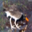
\includegraphics[width=31mm]{figures/cifar_ambiguous_input.png}}
\put(19.5,1){\makebox(0,3)}
\put(46,25){\makebox(0,3)[c]{\small}}
\put(39,21){\vector(1,0){15}}
\put(68,33.0){\makebox(0,3)[r]{\fontsize{9}{10}\selectfont airplane}}
\put(70,33.5){\textcolor{introblue}{\rule{1.52816322mm}{2.1mm}}}
\put(68,29.5){\makebox(0,3)[r]{\fontsize{9}{10}\selectfont automobile}}
\put(70,30.0){\textcolor{introblue}{\rule{1.52816322mm}{2.1mm}}}
\put(68,26.0){\makebox(0,3)[r]{\fontsize{9}{10}\selectfont bird}}
\put(70,26.5){\textcolor{introblue}{\rule{15.42340682mm}{2.1mm}}}
\put(68,22.5){\makebox(0,3)[r]{\fontsize{9}{10}\selectfont cat}}
\put(70,23.0){\textcolor{introblue}{\rule{1.53256924mm}{2.1mm}}}
\put(68,19.0){\makebox(0,3)[r]{\fontsize{9}{10}\selectfont deer}}
\put(70,19.5){\textcolor{introblue}{\rule{6.96360553mm}{2.1mm}}}
\put(68,15.5){\makebox(0,3)[r]{\fontsize{9}{10}\selectfont dog}}
\put(70,16.0){\textcolor{introblue}{\rule{1.53611694mm}{2.1mm}}}
\put(68,12.0){\makebox(0,3)[r]{\fontsize{9}{10}\selectfont frog}}
\put(70,12.5){\textcolor{lmugreen}{\rule{16.77271626mm}{2.1mm}}}
\put(68,8.5){\makebox(0,3)[r]{\fontsize{9}{10}\selectfont horse}}
\put(70,9.0){\textcolor{introblue}{\rule{1.52816322mm}{2.1mm}}}
\put(68,5.0){\makebox(0,3)[r]{\fontsize{9}{10}\selectfont ship}}
\put(70,5.5){\textcolor{introblue}{\rule{1.52816322mm}{2.1mm}}}
\put(68,1.5){\makebox(0,3)[r]{\fontsize{9}{10}\selectfont truck}}
\put(70,2.0){\textcolor{introblue}{\rule{1.65893229mm}{2.1mm}}}
\put(70,0.5){\line(1,0){50}}
\put(70,0.5){\line(0,-1){.7}}
\put(70,-3.8){\makebox(0,3)[c]{\small 0}}
\put(95.0,0.5){\line(0,-1){.7}}
\put(95.0,-3.8){\makebox(0,3)[c]{\small 0.5}}
\put(120,0.5){\line(0,-1){.7}}
\put(120,-3.8){\makebox(0,3)[c]{\small 1}}
\put(95,-7){\makebox(0,3)[c]{\small Class probability}}
\end{picture}
